\chapter{Catene Di Markov}

\begin{quote}
    \itshape Non si può discendere due volte nello stesso fiume, né toccare due volte una sostanza nel medesimo stato
\end{quote}

\section{Variabili Aleatorie Discrete}

Per comprendere appieno le Catene di Markov, è necessario richiamare i concetti fondamentali relativi alle variabili aleatorie discrete e alle loro distribuzioni di probabilità.


\subsubsection{Spazio di probabilità}

Uno \emph{spazio di probabilità} è una terna

$$
(\Omega,\mathcal{F},P)
$$

formata da tre componenti fondamentali:

\begin{itemize}
\item $\Omega$ è lo \textbf{spazio campionario}, cioè l'insieme di tutti i possibili risultati di un esperimento casuale;

\item $\mathcal{F}$ è una \textbf{$\sigma$-algebra di eventi} (\textbf{la proprietà fondamentale che devi sapere della sigma-algebra di eventi è che $\Omega \in \mathcal{F}$}), cioè una collezione di sottoinsiemi di $\Omega$ ai quali è possibile assegnare una probabilità;

\begin{equation}
    \mathcal{F} \subseteq P(\Omega)
\end{equation}

\item $P$ è la \textbf{misura di probabilità}, cioè una funzione che assegna a ogni evento $A\in\mathcal{F}$ un valore compreso tra $0$ e $1$:
\[
P:\mathcal{F}\rightarrow[0,1].
\]

\end{itemize}

\paragraph{Spazio campionario $\Omega$}

Lo spazio campionario $\Omega$ contiene tutti gli esiti possibili dell'esperimento casuale.

Ad esempio, considerando il lancio di un dado a sei facce:

$$
\Omega=\{1,2,3,4,5,6\}.
$$

Ogni elemento $\omega\in\Omega$ rappresenta un possibile risultato dell'esperimento.

\paragraph{Insieme degli eventi $\mathcal{F}$}

Un \emph{evento} è un sottoinsieme dello spazio campionario $\Omega$. L'insieme $\mathcal{F}$ raccoglie gli eventi ai quali possiamo assegnare una probabilità.

Ad esempio, nel lancio di un dado, consideriamo l'evento

$$
A=\{2,4,6\},
$$

che rappresenta l'evento ``esce un numero pari''. In questo caso:

$$
A\in\mathcal{F}.
$$

Formalmente, $\mathcal{F}$ è una $\sigma$-algebra su $\Omega$.


\paragraph{Misura di probabilità $P$}

La funzione

$$
P:\mathcal{F}\rightarrow[0,1]
$$

assegna a ogni evento $A\in\mathcal{F}$ una probabilità.

Ad esempio, se il dado è equo:

$$
P(\{2\})=\frac{1}{6}
$$

mentre per l'evento ``esce un numero pari'':

$$
P(\{2,4,6\})=\frac{3}{6}=\frac{1}{2}.
$$

La misura di probabilità soddisfa, tra le altre, le proprietà:

$$
P(\Omega)=1
$$

e

$$
P(A)\geq 0
\qquad\forall A\in\mathcal{F}.
$$

In sintesi:

$$
\boxed{
\Omega=\text{possibili risultati}
}
$$

$$
\boxed{
\mathcal{F}=\text{eventi ai quali assegniamo una probabilità}
}
$$

$$
\boxed{
P=\text{probabilità assegnata agli eventi}
}
$$

\subsubsection*{Variabile aleatoria}

Una \emph{variabile aleatoria} è una funzione che associa a ogni possibile risultato $\omega\in\Omega$ un valore numerico.

Formalmente:

$$
\boxed{X:\Omega\rightarrow\mathbb{R}}
$$

e quindi:

$$
\omega\in\Omega
\quad\xrightarrow{\quad X\quad}\quad
X(\omega)\in\mathbb{R}.
$$

La variabile aleatoria permette quindi di trasformare gli esiti dell'esperimento casuale in valori numerici sui quali possiamo effettuare operazioni matematiche.

\paragraph{Esempio: lancio di un dado}

Consideriamo nuovamente:

$$
\Omega=\{1,2,3,4,5,6\}.
$$

Possiamo definire una variabile aleatoria $X$ come

$$
X(\omega)=\omega.
$$

In questo caso la variabile aleatoria restituisce semplicemente il valore uscito dal dado:

$$
\begin{array}{c|cccccc}
\omega & 1 & 2 & 3 & 4 & 5 & 6\\
\hline
X(\omega) & 1 & 2 & 3 & 4 & 5 & 6
\end{array}
$$

Possiamo però definire anche una variabile aleatoria diversa. Ad esempio:

$$
X(\omega)=
\begin{cases}
1 & \text{se }\omega\text{ è pari},\\
0 & \text{se }\omega\text{ è dispari}.
\end{cases}
$$

In questo caso:

$$
\begin{array}{c|cccccc}
\omega & 1 & 2 & 3 & 4 & 5 & 6\\
\hline
X(\omega) & 0 & 1 & 0 & 1 & 0 & 1
\end{array}
$$

Quindi, se ad esempio il dado restituisce $\omega=4$, si ha:

$$
X(4)=1.
$$

L'idea fondamentale può essere rappresentata come:

$$
\boxed{
\text{esperimento casuale}
\longrightarrow
\omega\in\Omega
\longrightarrow
X(\omega)\in\mathbb{R}
}
$$

La variabile aleatoria permette quindi di associare un valore numerico a ciascun possibile esito dell'esperimento. Questo consente successivamente di definire e studiare la sua \emph{distribuzione di probabilità}, il \emph{valore atteso}, la \emph{varianza} e altre quantità statistiche.



\subsection{Definizione e Supporto}

\begin{definition}{Variabile Aleatoria Discreta}
Sia $(\Omega, \mathcal{F}, \mathcal{P})$ uno spazio di probabilità. Una \textbf{variabile aleatoria} (v.a.) discreta $X$ è una funzione misurabile:
\[
X: \Omega \longrightarrow S \subset \mathbb{R}
\]
tale che l'insieme immagine $S$ (detto \textbf{supporto} o spazio dei valori assunti da $X$) sia finito oppure numerabile:
\[
S = \{s_1, s_2, s_3, \dots\}
\]
\end{definition}

Nel contesto dei sistemi dinamici e delle catene di Markov, $X$ rappresenta tipicamente lo \emph{stato} del sistema rilevato in un determinato istante temporale.

\subsection{Funzione di Massa di Probabilità (PMF)}

La distribuzione di probabilità di una variabile aleatoria discreta $X$ è completamente caratterizzata dalla sua \textbf{Funzione di Massa di Probabilità} (PMF, \emph{Probability Mass Function}), indicata con $p_X(x)$:

\[
p_X : S \to [0,1]
\]

La PMF è definita in questo modo, quella che fa è prendere gli insiemi di valori che la variabile aleatoria $X$ può assumere e assegnare un numero compreso fra 0 e 1.
\textbf{Quindi intuitivamente quello che fa è dire quanta probabilità ha la variabile aleatoria di assumere quel valore}.
Questa è definita cosi:

\[
p_X(x) = \mathcal{P}(X = x) \quad \text{per ogni } x \in S
\]

La PMF rispetta due proprietà fondamentali degli assiomi di Kolmogorov:
\begin{enumerate}
    \item \textbf{Non negatività}: $p_X(s_k) \ge 0 \quad \forall s_k \in S$
    \item \textbf{Normalizzazione}: $\sum_{s_k \in S} p_X(s_k) = 1$
\end{enumerate}


\begin{warning}
    Nota che la funzione $P$ definita nella tripla dello spazio di campionamento, prende in ingresso, un evento sottoinsieme di $\mathcal{F}$,
    e infatti $X=x$, rappresenta un evento di $\mathcal{F}$, perchè:
    \begin{equation}
        \{\omega \in \Omega : X(\omega) = x\}
    \end{equation}
\end{warning}

\subsubsection{Esempio Variabile Aleatoria}

Consideriamo lo spazio di probabilità

\[
\Omega = \{1,2,3,4,5,6\},
\]

che rappresenta il lancio di un dado a sei facce, con tutti gli esiti equiprobabili:

\[
P(\{\omega\}) = \frac{1}{6},
\qquad \forall \omega \in \Omega.
\]

Definiamo la variabile aleatoria

\[
X:\Omega \to S
\]

come

\[
X(\omega)=
\begin{cases}
1 & \text{se } \omega \text{ è pari},\\
0 & \text{se } \omega \text{ è dispari}.
\end{cases}
\]

In particolare:

\[
\begin{array}{c|cccccc}
\omega & 1 & 2 & 3 & 4 & 5 & 6\\
\hline
X(\omega) & 0 & 1 & 0 & 1 & 0 & 1
\end{array}
\]

Pertanto, l'insieme dei possibili valori assunti da \(X\) è

\[
S=\{0,1\}.
\]

La \emph{PMF} (Probability Mass Function) di $X$ è la funzione

\[
p_X:S\to[0,1],
\]

definita come

\[
p_X(x)=P(X=x).
\]

Nel nostro caso:

\[
p_X(0)=P(X=0)
=P(\{1,3,5\})=P(\{1\} \cup \{2\} \cup \{3\}) = P(\{1\}) + P(\{2\}) + P(\{3\})
=\frac{3}{6}
=\frac12,
\]

mentre

\[
p_X(1)=P(X=1)
=P(\{2,4,6\})
=\frac{3}{6}
=\frac12.
\]

Quindi la PMF è

\[
\boxed{
p_X(x)=
\begin{cases}
\frac12 & x=0,\\
\frac12 & x=1,\\
0 & \text{altrimenti}.
\end{cases}}
\]

Si osserva che la PMF soddisfa le due proprietà fondamentali:

\[
p_X(x)\geq 0
\qquad \forall x\in S
\]

e

\[
\sum_{x\in S}p_X(x)
=
p_X(0)+p_X(1)
=
\frac12+\frac12
=1.
\]



\subsection{Probabilità Condizionata e Distribuzioni Congiunte}

Quando si studiano le relazioni tra più variabili aleatorie (ad esempio, lo stato $X_t$ al tempo $t$ e lo stato $X_{t+1}$ al tempo $t+1$), si utilizzano la distribuzione congiunta e la probabilità condizionata.

\begin{definition}{Probabilità Condizionata}
Dati due eventi $A, B \in \mathcal{F}$ con $\mathcal{P}(B) > 0$, la probabilità condizionata di $A$ dato $B$ è definita come:
\[
\mathcal{P}(A \mid B) = \frac{\mathcal{P}(A \cap B)}{\mathcal{P}(B)}
\]
\end{definition}

\subsection{PMF congiunta}

Consideriamo due variabili aleatorie discrete

$$
X:\Omega\to S_X,
\qquad
Y:\Omega\to S_Y.
$$

La \emph{PMF congiunta} (Probability Mass Function congiunta) di $X$ e $Y$ descrive la probabilità che le due variabili assumano contemporaneamente determinati valori.

Si definisce come

$$
\boxed{
p_{X,Y}(x,y)
=
P(X=x,Y=y)
}
$$

per ogni

$$
x\in S_X,\qquad y\in S_Y.
$$

In altre parole,

$$
p_{X,Y}(x,y)
$$

è la probabilità dell'evento in cui contemporaneamente

$$
X=x
$$

e

$$
Y=y.
$$

L'evento corrispondente è infatti
$$
\{X=x\}\cap\{Y=y\}.
$$

\subsubsection{Proprietà della PMF congiunta}

Essendo una PMF, $p_{X,Y}$ deve soddisfare due proprietà fondamentali.

\paragraph{1. Non negatività}

Per ogni coppia $(x,y)$:

$$
\boxed{
p_{X,Y}(x,y)\geq 0
}
$$

poiché rappresenta una probabilità.

\paragraph{2. Somma uguale a uno}

La somma della PMF congiunta su tutti i possibili valori di $X$ e $Y$ deve essere uguale a $1$:

$$
\boxed{
\sum_{x\in S_X}\sum_{y\in S_Y}
p_{X,Y}(x,y)=1
}
$$

Questo perché le coppie $(x,y)$ comprendono tutti i possibili valori che le due variabili possono assumere.

\subsubsection{Esempio}

Supponiamo che la PMF congiunta di $X$ e $Y$ sia descritta dalla seguente tabella:

$$
\begin{array}{c|ccc}
p_{X,Y}(x,y) & Y=0 & Y=1 & Y=2\\
\hline
X=0 & \frac{1}{8} & \frac{1}{8} & \frac{1}{4}\\
X=1 & \frac{1}{8} & \frac{1}{4} & \frac{1}{8}
\end{array}
$$

La somma di tutte le probabilità è

$$
\frac18+\frac18+\frac14+
\frac18+\frac14+\frac18=1.
$$

Per esempio,

$$
p_{X,Y}(1,2)
=
P(X=1,Y=2)
=
\frac18.
$$

Quindi la PMF congiunta permette di conoscere la probabilità di ogni possibile combinazione dei valori di $X$ e $Y$.

\subsubsection{PMF marginali}

Dalla PMF congiunta possiamo ottenere le distribuzioni delle singole variabili aleatorie.

La PMF marginale di $X$ si ottiene sommando la PMF congiunta rispetto a tutti i possibili valori di $Y$:

$$
\boxed{
p_X(x)
=
\sum_{y\in S_Y}p_{X,Y}(x,y)
}
$$

Analogamente, la PMF marginale di $Y$ si ottiene sommando rispetto a tutti i possibili valori di $X$:

$$
\boxed{
p_Y(y)
=
\sum_{x\in S_X}p_{X,Y}(x,y)
}
$$

Nel nostro esempio:

$$
p_X(0)
=
\frac18+\frac18+\frac14
=
\frac12
$$

e

$$
p_X(1)
=
\frac18+\frac14+\frac18
=
\frac12.
$$

Analogamente,

$$
p_Y(0)
=
\frac18+\frac18
=
\frac14,
$$

$$
p_Y(1)
=
\frac18+\frac14
=
\frac38,
$$

e

$$
p_Y(2)
=
\frac14+\frac18
=
\frac38.
$$

Quindi la PMF congiunta contiene abbastanza informazioni da permettere di ricostruire le PMF marginali delle singole variabili.

\subsubsection{PMF condizionata}

Possiamo anche studiare la distribuzione di una variabile aleatoria sapendo che l'altra ha assunto un determinato valore.

La PMF di $Y$ condizionata dall'evento ${X=x}$ è definita come

$$
\boxed{
p_{Y\mid X}(y\mid x)
=
P(Y=y\mid X=x)
}
$$

e, per $P(X=x)>0$,

$$
\boxed{
p_{Y\mid X}(y\mid x)
=
\frac{P(X=x,Y=y)}
{P(X=x)}
}
$$

ossia

$$
\boxed{
p_{Y\mid X}(y\mid x)
=
\frac{p_{X,Y}(x,y)}
{p_X(x)}
}
$$

Questa formula è semplicemente la definizione di probabilità condizionata applicata agli eventi

$$
\{Y=y\}
$$

e

$$
\{X=x\}.
$$

\subsubsection{Esempio di PMF condizionata}

Consideriamo nuovamente la tabella precedente e calcoliamo

$$
P(Y=1\mid X=0).
$$

Abbiamo

$$
p_{X,Y}(0,1)=\frac18
$$

e

$$
p_X(0)=\frac12.
$$

Pertanto:

$$
p_{Y\mid X}(1\mid0)
=
\frac{p_{X,Y}(0,1)}
{p_X(0)}
=
\frac{\frac18}{\frac12}
=
\frac14.
$$

Quindi, sapendo che

$$
X=0,
$$

la probabilità che

$$
Y=1
$$

è

$$
\boxed{
P(Y=1\mid X=0)=\frac14.
}
$$

\subsubsection{Proprietà della PMF condizionata}

Anche la PMF condizionata è una PMF. Pertanto deve soddisfare:

$$
p_{Y\mid X}(y\mid x)\geq0
$$

e, fissato un valore $x$ con $p_X(x)>0$,

$$
\boxed{
\sum_{y\in S_Y}
p_{Y\mid X}(y\mid x)=1.
}
$$

Quindi, una volta fissato $X=x$, le probabilità condizionate di tutti i possibili valori di $Y$ devono sommare a $1$.



\subsection{Esempio di probabilità congiunta con variabili aleatorie}

Consideriamo il lancio di due monete equilibrate. Definiamo lo spazio di probabilità

$$
(\Omega,\mathcal{F},P).
$$

Lo spazio di campionamento è

$$
\Omega=\{TT,TC,CT,CC\},
$$

dove:
\begin{itemize}
\item $T$ indica testa;
\item $C$ indica croce.
\end{itemize}

L'insieme degli eventi è

$$
\mathcal{F}=2^\Omega,
$$

cioè l'insieme di tutti i sottoinsiemi di $\Omega$.

Poiché le due monete sono equilibrate e indipendenti, ogni esito elementare ha probabilità

$$
P(\{\omega\})=\frac14,
\qquad \forall\omega\in\Omega.
$$

Ricordiamo però, che :
\begin{equation}
    F=\{\varnothing,\{TT\},\{TC\},\ldots,\{TT,TC,CT,CC\}\},
\end{equation}
E $P$ è definita su $F$, quindi poi $P$, assegnando le probabilità agli eventi \{TT,CC,CT,TC\}, riesce ad assegnare una probabilità a tutti gli eventi:
\newpage
\[
P({TT,TC})=P({TT})+P({TC})=\frac{1}{2}
\]
$\dots$
\[
P(\Omega)=1
\]



Definiamo ora due variabili aleatorie discrete:

$$
X:\Omega\to\{0,1,2\}
$$

e

$$
Y:\Omega\to\{0,1\}.
$$

La variabile $X$ rappresenta il numero totale di teste ottenute, mentre $Y$ indica se la prima moneta è testa:

$$
X(\omega)=
\begin{cases}
2 & \text{se ci sono due teste},\\
1 & \text{se c'è una sola testa},\\
0 & \text{se non ci sono teste},
\end{cases}
$$

e

$$
Y(\omega)=
\begin{cases}
1 & \text{se la prima moneta è testa},\\
0 & \text{se la prima moneta è croce}.
\end{cases}
$$

Possiamo rappresentare i valori delle due variabili nella seguente tabella:

$$
\begin{array}{c|cccc}
\omega & TT & TC & CT & CC\\
\hline
X(\omega) & 2 & 1 & 1 & 0\\
Y(\omega) & 1 & 1 & 0 & 0
\end{array}
$$

Consideriamo ora la probabilità congiunta

$$
P(X=1,Y=0).
$$

Questa espressione indica la probabilità che si verifichino
\emph{contemporaneamente} i due eventi:

$$
X=1
$$

e

$$
Y=0.
$$

In termini di eventi appartenenti a $\mathcal F$:

$$
\{X=1\}=\{TC,CT\}
$$

mentre

$$
\{Y=0\}=\{CT,CC\}.
$$

Pertanto:

$$
\{X=1\}\cap\{Y=0\}
=
\{CT\}.
$$

Di conseguenza,

$$
P(X=1,Y=0)
=
P(\{CT\})
=
\frac14.
$$

Questa probabilità è un esempio di \emph{probabilità congiunta}.

Possiamo quindi definire la PMF congiunta di $X$ e $Y$ come

$$
p_{X,Y}(x,y)
=
P(X=x,Y=y).
$$

Nel nostro esempio otteniamo:

$$
\begin{array}{c|cc}
p_{X,Y}(x,y) & Y=0 & Y=1\\
\hline
X=0 & \frac14 & 0\\
X=1 & \frac14 & \frac14\\
X=2 & 0 & \frac14
\end{array}
$$

Ad esempio:

$$
p_{X,Y}(1,0)
=
P(X=1,Y=0)
=
\frac14.
$$

Analogamente:

$$
p_{X,Y}(1,1)
=
P(X=1,Y=1)
=
P(\{TC\})
=
\frac14.
$$

Notiamo che la somma di tutte le probabilità della PMF congiunta è uguale a $1$:

$$
\sum_x\sum_y p_{X,Y}(x,y)
=
\frac14+\frac14+\frac14+\frac14
=
1.
$$

Quindi la PMF congiunta descrive la probabilità di tutte le possibili combinazioni dei valori assunti contemporaneamente da $X$ e $Y$.



\subsubsection{Esempio di Probabilità Condizionata}

Consideriamo uno spazio di probabilità

\[
(\Omega,\mathcal{F},P),
\]

dove lo spazio di campionamento è

\[
\Omega=\{TT,TC,CT,CC\},
\]

con:
\begin{itemize}
    \item $T$ = testa;
    \item $C$ = croce.
\end{itemize}

Supponiamo che le due monete siano equilibrate e indipendenti. 
L'insieme degli eventi è

\[
\mathcal{F}=2^\Omega,
\]

cioè l'insieme di tutti i sottoinsiemi di $\Omega$.

Poiché i quattro risultati sono equiprobabili,

\[
P(\{\omega\})=\frac14,
\qquad \forall \omega\in\Omega.
\]

Definiamo ora due variabili aleatorie:

\[
X:\Omega\to\{0,1,2\},
\]

dove $X$ rappresenta il numero di teste ottenute, e

\[
Y:\Omega\to\{0,1\},
\]

dove $Y$ indica se la prima moneta è testa:

\[
Y(\omega)=
\begin{cases}
1 & \text{se la prima moneta è testa},\\
0 & \text{altrimenti}.
\end{cases}
\]

La variabile $X$ assume i seguenti valori:

\[
\begin{array}{c|cccc}
\omega & TT & TC & CT & CC\\
\hline
X(\omega) & 2 & 1 & 1 & 0\\
Y(\omega) & 1 & 1 & 0 & 0
\end{array}
\]

Consideriamo ora la probabilità condizionata

\[
P(X=2\mid Y=1).
\]

Per definizione,

\[
P(X=2\mid Y=1)
=
\frac{P(X=2\cap Y=1)}
{P(Y=1)},
\]

purché $P(Y=1)>0$.

Osserviamo che

\[
\{X=2\}=\{TT\}
\]

mentre

\[
\{Y=1\}=\{TT,TC\}.
\]

Inoltre,

\[
\{X=2\}\cap\{Y=1\}
=
\{TT\}.
\]

Pertanto:

\[
P(X=2\cap Y=1)
=
P(\{TT\})
=
\frac14
\]

e

\[
P(Y=1)
=
P(\{TT,TC\})
=
\frac24
=
\frac12.
\]

Quindi:

\[
\boxed{
P(X=2\mid Y=1)
=
\frac{\frac14}{\frac12}
=
\frac12
}
\]

In altre parole, sapendo che la prima moneta è risultata testa, la probabilità di ottenere due teste è $\frac12$.


\subsection{Dai Processi Stocastici alle Sequenze Temporali}

Un \textbf{processo stocastico a tempo discreto} è una famiglia indicizzata di variabili aleatorie:
\[
\{X_t\}_{t \in \mathbb{N}_0} = \{X_0, X_1, X_2, \dots\}
\]
definite sullo stesso spazio di probabilità, dove l'indice $t$ rappresenta il tempo e $X_t$ descrive lo stato del sistema all'istante $t$. 

In generale, la distribuzione probabilistica di $X_{t+1}$ potrebbe dipendere dall'intera storia passata del processo, ossia dai valori assunti da $X_0, X_1, \dots, X_t$. Le \emph{Catene di Markov} semplificano questa dipendenza mediante un'ipotesi fondamentale.

\newpage

\section{Catene di Markov}

\subsection{Introduzione e Proprietà di Assenza di Memoria}

Una \textbf{catena di Markov a tempo discreto} è un particolare tipo di processo stocastico. Consideriamo uno spazio di probabilità

$$
(\Omega,\mathcal{F},P),
$$

dove $\Omega$ è lo spazio campionario, $\mathcal{F}$ è una $\sigma$-algebra di eventi e $P$ è la misura di probabilità definita su $\mathcal{F}$.

Un processo stocastico a tempo discreto è una famiglia di variabili aleatorie

$$
\{X_t\}_{t\in\mathbb{N}_0}
=
\{X_0,X_1,X_2,\ldots\},
$$

tutte definite sullo stesso spazio di probabilità $(\Omega,\mathcal{F},P)$.

Per ogni istante $t$, la variabile aleatoria

$$
X_t:\Omega\longrightarrow S
$$

associa a ogni esito $\omega\in\Omega$ lo stato assunto dal sistema all'istante $t$. L'insieme $S$ è detto \textbf{spazio degli stati} e contiene tutti i possibili valori che il processo può assumere. Nel caso di una catena di Markov a stati discreti possiamo scrivere

$$
S=\{s_1,s_2,\ldots\}.
$$

Pertanto, fissato un esito $\omega\in\Omega$, la successione

$$
X_0(\omega),X_1(\omega),X_2(\omega),\ldots
$$

descrive l'evoluzione del sistema nel tempo per quell'esito.

In generale, la distribuzione probabilistica dello stato futuro $X_{t+1}$ potrebbe dipendere dall'intera storia del processo, ossia dai valori

$$
X_0,X_1,\ldots,X_t.
$$

Le catene di Markov introducono una particolare ipotesi, detta \textbf{proprietà di Markov} o \textbf{proprietà di assenza di memoria}: \textbf{una volta noto lo stato attuale $X_t$, la conoscenza degli stati precedenti non fornisce ulteriori informazioni sullo stato futuro $X_{t+1}$.}

Formalmente, per ogni $t\in\mathbb{N}_0$ e per ogni $s_0,\ldots,s_t,s_{t+1}\in S$,

$$
\boxed{
P
\left(
X_{t+1}=s_{t+1}
\mid
X_t=s_t,X_{t-1}=s_{t-1},\ldots,X_0=s_0
\right)
=
P
\left(
X_{t+1}=s_{t+1}
\mid
X_t=s_t
\right)
}
$$

La proprietà di Markov afferma quindi che, \textbf{per prevedere probabilisticamente lo stato successivo, è sufficiente conoscere lo stato attuale: la storia precedente del processo può essere ignorata}.

Quindi questa proprietà ci dice che:
\begin{center}
    Una volta noto lo stato attuale,\textbf{la conoscenza degli stati precedenti non fornisce ulteriori informazioni sullo stato futuro}
\end{center}

\subsection{Spazio degli Stati e Tempo Discreto}

In realtà, la maggior parte dei fenomeni fisici e dei sistemi di interesse sono di fatto modellabili come catene di Markov. Chiaramente, da dominio a dominio, vi sono diverse varianti che dipendono dallo spazio degli stati in cui il sistema si può trovare, dalla natura del tempo, ecc.

Nel nostro contesto assumiamo che:
\begin{itemize}
    \item L'insieme degli stati $S$ sia \textbf{finito} di cardinalità $n$: 
    \[
    S = \{s_1, s_2, \dots, s_n\}
    \]
    \item Il \textbf{tempo sia discreto}: $t \in \{0, 1, 2, \dots\}$.
\end{itemize}

\subsection{Matrice delle Transizioni}

Una catena di Markov a tempo discreto e spazio degli stati finito può essere rappresentata da una \textbf{matrice delle transizioni} $P$ di dimensione $n \times n$, tale che l'elemento $p_{i,j}$ della matrice corrisponde alla probabilità che il sistema transiti da uno stato $s_i$ ad uno stato $s_j$:

\[
p_{i,j} = \mathcal{P}(x_{t+1} = s_j \mid x_t = s_i)
\]

dove la variabile aleatoria $x_t$ indica lo stato del sistema al tempo $t$.

\subsection{Struttura della Matrice di Transizione}

La matrice di transizione $P$ ha la seguente struttura formale :
\[
P = \begin{pmatrix}
p_{1,1} & p_{1,2} & \cdots & p_{1,n} \\
p_{2,1} & p_{2,2} & \cdots & p_{2,n} \\
\vdots & \vdots & \ddots & \vdots \\
p_{n,1} & p_{n,2} & \cdots & p_{n,n}
\end{pmatrix}
\]

\textbf{Questa matrice la puoi vedere anche come la matrice di transazione al tempo $t$}

Essa soddisfa le seguenti proprietà fondanti (matrice stocastica per righe):
\begin{enumerate}
    \item Tutti gli elementi sono probabilità valide:
    \[
    p_{i,j} \ge 0 \quad \forall i, j \in \{1, \dots, n\}
    \]
    \item La somma di ogni riga è pari ad $1$ (proprietà della pmf condizionata):
    \[
    \sum_{j=1}^{n} p_{i,j} = 1 \quad \forall i \in \{1, \dots, n\}
    \]
\end{enumerate}

\subsection{Evoluzione della Distribuzione di Probabilità}

Consideriamo una catena di Markov a tempo discreto con spazio degli stati finito

\[
S = \{s_1,s_2,\dots,s_n\}.
\]

Al tempo $t$, la variabile aleatoria $X_t$ descrive lo stato in cui si trova il sistema. La distribuzione di probabilità dello stato al tempo $t$ può essere rappresentata mediante il vettore

\[
\mu^t =
\begin{pmatrix}
\mu_1^t & \mu_2^t & \cdots & \mu_n^t
\end{pmatrix},
\]

dove

\[
\mu_i^t = \mathcal{P}(X_t=s_i).
\]

Pertanto, il vettore $\mu^t$ contiene le probabilità che il sistema si trovi nei diversi stati al tempo $t$ e, essendo una distribuzione di probabilità, soddisfa

\[
\sum_{i=1}^{n}\mu_i^t=1.
\]

L'obiettivo è determinare la distribuzione del sistema al tempo successivo $t+1$, ovvero calcolare

\[
\mu_j^{t+1}
=
\mathcal{P}(X_{t+1}=s_j).
\]

Per raggiungere lo stato $s_j$ al tempo $t+1$, il sistema deve necessariamente trovarsi in uno degli stati $s_1,\dots,s_n$ al tempo $t$. Possiamo quindi applicare il \textbf{teorema della probabilità totale}:

\[
\mathcal{P}(X_{t+1}=s_j)
=
\sum_{i=1}^{n}
\mathcal{P}(X_{t+1}=s_j,X_t=s_i).
\]

Utilizzando la definizione di probabilità condizionata,

\[
\mathcal{P}(A\cap B)
=
\mathcal{P}(A\mid B)\mathcal{P}(B),
\]

otteniamo

\[
\mathcal{P}(X_{t+1}=s_j)
=
\sum_{i=1}^{n}
\mathcal{P}(X_{t+1}=s_j\mid X_t=s_i)
\mathcal{P}(X_t=s_i).
\]

Per la definizione della distribuzione $\mu^t$,

\[
\mathcal{P}(X_t=s_i)=\mu_i^t,
\]

mentre, per la definizione della matrice di transizione,

\[
\mathcal{P}(X_{t+1}=s_j\mid X_t=s_i)=p_{i,j}.
\]

Pertanto,

\[
\boxed{
\mu_j^{t+1}
=
\sum_{i=1}^{n}p_{i,j}\mu_i^t
}
\]

Questa relazione mostra come la distribuzione di probabilità del sistema si evolve da un istante temporale al successivo.

\subsubsection{Interpretazione della formula}

La quantità

\[
p_{i,j}\mu_i^t
\]

può essere interpretata come la probabilità di seguire il seguente percorso:

\[
\text{essere nello stato }s_i\text{ al tempo }t
\quad\longrightarrow\quad
\text{passare allo stato }s_j\text{ al tempo }t+1.
\]

Infatti,

\[
\mu_i^t=\mathcal{P}(X_t=s_i)
\]

rappresenta la probabilità di trovarsi nello stato $s_i$ al tempo $t$, mentre

\[
p_{i,j}
=
\mathcal{P}(X_{t+1}=s_j\mid X_t=s_i)
\]

rappresenta la probabilità di passare da $s_i$ a $s_j$.

Per ottenere la probabilità complessiva di trovarsi in $s_j$ al tempo $t+1$, dobbiamo considerare tutti i possibili stati di partenza $s_i$ e sommare i relativi contributi:

\[
\mu_j^{t+1}
=
p_{1,j}\mu_1^t
+
p_{2,j}\mu_2^t
+\cdots+
p_{n,j}\mu_n^t.
\]

\subsubsection{Forma matriciale}

La relazione precedente può essere espressa in forma matriciale in modo molto più compatto.

Consideriamo il vettore riga

\[
\mu^t=
\begin{pmatrix}
\mu_1^t & \mu_2^t & \cdots & \mu_n^t
\end{pmatrix}
\]

e la matrice di transizione

\[
P=
\begin{pmatrix}
p_{1,1} & p_{1,2} & \cdots & p_{1,n}\\
p_{2,1} & p_{2,2} & \cdots & p_{2,n}\\
\vdots & \vdots & \ddots & \vdots\\
p_{n,1} & p_{n,2} & \cdots & p_{n,n}
\end{pmatrix}.
\]

Il prodotto $\mu^tP$ produce un nuovo vettore riga le cui componenti sono

\[
(\mu^tP)_j
=
\sum_{i=1}^{n}\mu_i^t p_{i,j}.
\]

Ma abbiamo appena dimostrato che

\[
\mu_j^{t+1}
=
\sum_{i=1}^{n}p_{i,j}\mu_i^t.
\]

Pertanto,

\[
\boxed{
\mu^{t+1}=\mu^tP
}
\]

Questa equazione rappresenta l'evoluzione della distribuzione di probabilità della catena di Markov da un istante al successivo.

In particolare, possiamo interpretare la matrice $P$ come un operatore che, applicato alla distribuzione al tempo $t$, permette di ottenere la distribuzione al tempo $t+1$:

\[
\boxed{
\mu^t
\overset{P}{\longrightarrow}
\mu^{t+1}
}
\]

\subsubsection{Esempio}

Consideriamo una catena di Markov con due stati

\[
S=\{s_1,s_2\}.
\]

Supponiamo che al tempo $t$ la distribuzione sia

\[
\mu^t=
\begin{pmatrix}
0.7 & 0.3
\end{pmatrix},
\]

ossia

\[
\mathcal{P}(X_t=s_1)=0.7,
\qquad
\mathcal{P}(X_t=s_2)=0.3.
\]

Supponiamo inoltre che la matrice di transizione sia

\[
P=
\begin{pmatrix}
0.8 & 0.2\\
0.4 & 0.6
\end{pmatrix}.
\]

Ad esempio,

\[
p_{1,1}=0.8
\]

significa che

\[
\mathcal{P}(X_{t+1}=s_1\mid X_t=s_1)=0.8,
\]

mentre

\[
p_{2,1}=0.4
\]

significa che

\[
\mathcal{P}(X_{t+1}=s_1\mid X_t=s_2)=0.4.
\]

Calcoliamo la probabilità di trovarci nello stato $s_1$ al tempo $t+1$:

\[
\mu_1^{t+1}
=
p_{1,1}\mu_1^t+p_{2,1}\mu_2^t.
\]

Sostituendo i valori:

\[
\mu_1^{t+1}
=
0.8\cdot0.7+0.4\cdot0.3
=
0.56+0.12
=
0.68.
\]

Analogamente,

\[
\mu_2^{t+1}
=
p_{1,2}\mu_1^t+p_{2,2}\mu_2^t
\]

e quindi

\[
\mu_2^{t+1}
=
0.2\cdot0.7+0.6\cdot0.3
=
0.14+0.18
=
0.32.
\]

Di conseguenza,

\[
\mu^{t+1}
=
\begin{pmatrix}
0.68 & 0.32
\end{pmatrix}.
\]

Lo stesso risultato si ottiene direttamente mediante il prodotto matriciale:

\[
\mu^{t+1}
=
\mu^tP
=
\begin{pmatrix}
0.7&0.3
\end{pmatrix}
\begin{pmatrix}
0.8&0.2\\
0.4&0.6
\end{pmatrix}
=
\begin{pmatrix}
0.68&0.32
\end{pmatrix}.
\]

Quindi la matrice di transizione permette di trasformare la distribuzione di probabilità al tempo $t$ nella distribuzione al tempo $t+1$:

\[
\boxed{
\mu^{t+1}=\mu^tP
}
\]

\subsection{Distribuzioni Stazionarie}
Ricordati che vale questo:
\[
\begin{aligned}
\mu^1 &= \mu^0 P \\
\mu^2 &= \mu^1 P = \mu^0 P P \\
\dots \\
\mu^t &= \mu^{t-1} P = \mu^0 P^t
\end{aligned}
\]


Consideriamo la seguente matrice $P$, che si può vedere anche sottoforma di grafo:
\begin{figure}[htbp]
    \centering
    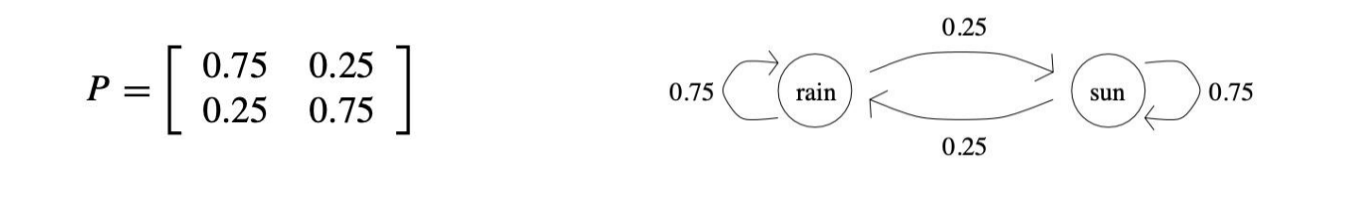
\includegraphics[width=0.7\textwidth]{_files/_images/mm1.png}
    \label{fig:etichetta}
\end{figure}

Consideriamo una distribuzione iniziale 
\[
\mu^{0}
=
\begin{pmatrix}
1  &  0
\end{pmatrix}.
\]
Allora avremo questo \textbf{random walk}:
\begin{figure}[htbp]
    \centering
    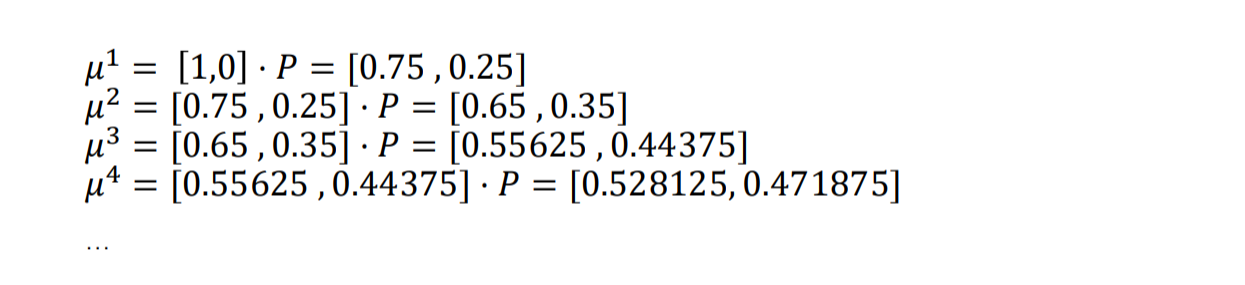
\includegraphics[width=0.4\textwidth]{_files/_images/mm2.png}
    \label{fig:etichetta}
\end{figure}

\newpage
Consideriamo una diversa distribuzione iniziale:
\[
\mu^{0}
=
\begin{pmatrix}
0.3  &  0.7
\end{pmatrix}
\]
Questa genera un random walk:
\begin{figure}[htbp]
    \centering
    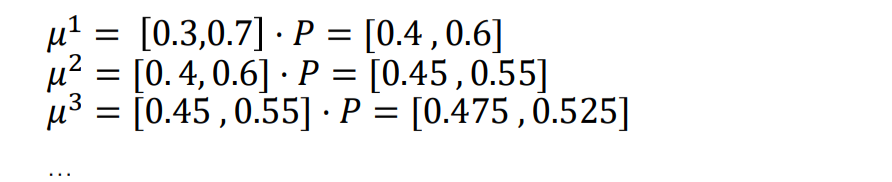
\includegraphics[width=0.4\textwidth]{_files/_images/mm3.png}
    \label{fig:etichetta}
\end{figure}

Come possiamo notare, sia la distribuzione 
\[
\mu^{0}
=
\begin{pmatrix}
0.3  &  0.7
\end{pmatrix}
\]
e 
\[
\mu^{0}
=
\begin{pmatrix}
1  &  0
\end{pmatrix}
\]
tendono alla distribuzione
\[
\begin{pmatrix}
0.5  &  0.5
\end{pmatrix}
\]

\textbf{Questa viene chiamata distribuzione stazionaria}, cioè una distribuzione tale che:
\begin{equation}
    \mu P = \mu
\end{equation}


Questo vale per ogni 
\[
\mu^{0}
=
\begin{pmatrix}
\alpha   &  1 - \alpha
\end{pmatrix} , \alpha \in [0,1]
\]
e dipende dal fatto che:
\[
\lim_{t \to \infty} P^t
=
\begin{bmatrix}
0.5 & 0.5 \\
0.5 & 0.5
\end{bmatrix}
\]

e quindi
\[
\lim_{t \to \infty} \mu^t
=
\lim_{t \to \infty} \mu^0 \cdot P^t
=
[0.5(\alpha + 1 - \alpha),\, 0.5(\alpha + 1 - \alpha)]
=
[0.5, 0.5].
\]

\textbf{Questo è un risultato specifico, di un teorema piu generale, chiamato Teorema Ergodico per le Catene di Markov}, il teorema dice che sotto determinata ipotesi,
quella di \textbf{Irriducibilità} e \textbf{Aperiodicità}, che vedremo dopo valgono:
\begin{itemize}
    \item \textbf{Struttura della matrice limite} : cioè la proprietà che abbiamo visto del limite della matrice, dove tutte le righe tendono alla distribuzione stazionaria.
    \item \textbf{Indipendenza dalla distribuzione iniziale}
    \item \textbf{Invarianza della distribuzione limite}
\end{itemize}
Dopo vedremo meglio queste 3 proprietà, vediamo nel dettaglio le 2 ipotesi che devono soddisfare la catena per far avvenire il teorema.

\subsubsection{Irriducibilità}

Sia $(S, P)$ una catena di Markov a tempo discreto definita su uno spazio degli stati finito $S = \{s_1, s_2, \dots, s_n\}$, descritta dalla matrice di transizione stocastica $P \in \mathbb{R}^{n \times n}$, le cui entrate rappresentano le probabilità di transizione in un singolo passo $P_{i,j} = \mathbb{P}(X_{t+1} = s_j \mid X_t = s_i)$.

\begin{definition}{Irriducibilità}
Una catena di Markov si dice \emph{irriducibile} se, per ogni coppia di stati $s_i, s_j \in S$, la probabilità di raggiungere $s_j$ da $s_i$ in un numero finito $t \ge 1$ di passi è strettamente positiva:
\begin{equation*}
\forall i, j \in \{1, \dots, n\}, \quad \exists t \ge 1 : P_{i,j}^t > 0
\end{equation*}
dove $P_{i,j}^t = (P^t)_{i,j}$ indica l'entrata $(i,j)$-esima della matrice di transizione elevata alla $t$-esima potenza, rappresentante le transizioni in $t$ passi, \textbf{cioè la probabilità di passare dallo stato $i$ allo stato $j$ in esattamente t passi}
\end{definition}
\begin{example}{Esempio}
Consideriamo una catena di Markov con spazio degli stati

$$
S=\{1,2\}
$$

e matrice di transizione

$$
P=
\begin{pmatrix}
0.5 & 0.5\\
0.2 & 0.8
\end{pmatrix}.
$$

Calcoliamo la matrice di transizione dopo due passi:

$$
P^2=P\cdot P
=
\begin{pmatrix}
0.35 & 0.65\\
0.26 & 0.74
\end{pmatrix}.
$$

La notazione

$$
P^2_{1,2}=(P^2)_{1,2}
$$

indica l'elemento della matrice $P^2$ che si trova alla riga $1$ e alla colonna $2$. Pertanto:

$$
P^2_{1,2}=0.65.
$$

Questo valore rappresenta la probabilità di passare dallo stato $1$ allo stato $2$ \emph{in esattamente due passi}.

Infatti, per arrivare da $1$ a $2$ in due passi sono possibili due percorsi:

$$
1\rightarrow1\rightarrow2
$$

oppure

$$
1\rightarrow2\rightarrow2.
$$

Le rispettive probabilità sono:

$$
P_{1,1}P_{1,2}=0.5\cdot0.5=0.25
$$

e

$$
P_{1,2}P_{2,2}=0.5\cdot0.8=0.40.
$$

Pertanto:

$$
P^2_{1,2}
=
P_{1,1}P_{1,2}
+
P_{1,2}P_{2,2}
=
0.25+0.40
=
0.65.
$$

In generale,

$$
\boxed{P^t_{i,j}=(P^t)_{i,j}}
$$

indica la probabilità di passare dallo stato $i$ allo stato $j$ in esattamente $t$ passi.
\end{example}


\paragraph{Interpretazione Grafo-Teorica}
Si consideri il grafo orientato delle transizioni $G = (V, E)$, dove $V = S$ e un arco orientato $(s_a, s_b) \in E$ sussiste se e solo se $P_{a,b} > 0$.\textbf{Cioè praticamente il grafo che abbiamo considerato anche prima, qui stiamo solo formalizzando il concetto}
\begin{itemize}
    \item Se non esiste alcun cammino orientato da $s_i$ a $s_j$ nel grafo $G$, allora per ogni $t \ge 1$ si ha $P_{i,j}^t = 0$.
    \item Se esiste un cammino orientato $s_i = v_0 \xrightarrow{\alpha_1} v_1 \xrightarrow{\alpha_2} \dots \xrightarrow{\alpha_m} v_m = s_j$ di lunghezza $m \ge 1$, con $P_{v_{h-1}, v_h} = \alpha_h > 0$, la probabilità della transizione lungo tale cammino soddisfa la disuguaglianza:
    \begin{equation*}
    P_{i,j}^m \ge \prod_{h=1}^m \alpha_h > 0 \implies P_{i,j}^m > 0
    \end{equation*}
\end{itemize}
Di conseguenza, la condizione di irriducibilità equivale alla proprietà di \emph{forte connessione} del grafo orientato $G$.

\begin{theorem}{Esistenza e Unicità della Distribuzione Stazionaria}
In virtù del Teorema di Perron-Frobenius per matrici non negative e irriducibili, se una catena di Markov è irriducibile, ammette una ed una sola distribuzione di probabilità stazionaria $\mu \in \mathbb{R}^{1 \times n}$, ovvero un vettore riga di probabilità tale che:
\begin{equation*}
\mu P = \mu \quad \text{con} \quad \sum_{i=1}^n \mu_i = 1 \quad \text{e} \quad \mu_i > 0, \quad \forall i \in \{1, \dots, n\}
\end{equation*}
\emph{Nota rigorosa:} L'irriducibilità garantisce l'unicità del punto fisso $\mu$, ma non implica necessariamente che una generica distribuzione iniziale $\mu_0$ converga a $\mu$ per $t \to \infty$. La convergenza richiede un'ulteriore proprietà algebrica e topologica: l'aperiodicità.
\end{theorem}

\subsubsection{Aperiodicità}

\begin{definition}{Insieme dei tempi di ritorno}
Sia $s_i \in S$ uno stato della catena di Markov. Si definisce l'insieme dei tempi di ritorno in $s_i$ come:
\begin{equation*}
A_i = \{ t \ge 1 \mid P_{i,i}^t > 0 \}
\end{equation*}
Quindi \(A_i\) contiene tutti i numeri di passi dopo i quali è possibile partire da \(s_i\) e ritornare in \(s_i\).
\textbf{è solitamente un insieme infinito}
\end{definition}

\begin{example}
Consideriamo una catena di Markov con spazio degli stati

$$
S=\{1,2\}
$$

e matrice di transizione

$$
P=
\begin{pmatrix}
0.5 & 0.5\\
0.5 & 0.5
\end{pmatrix}.
$$

Il grafo della catena è:

\begin{center}
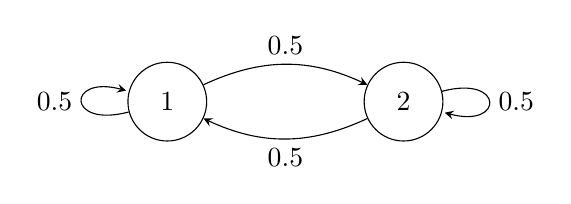
\begin{tikzpicture}[>=stealth, node distance=3cm]
\node[circle, draw, minimum size=1cm] (1) {$1$};
\node[circle, draw, minimum size=1cm, right of=1] (2) {$2$};


\draw[->, bend left=25] (1) to node[above] {$0.5$} (2);
\draw[->, bend left=25] (2) to node[below] {$0.5$} (1);

\draw[->] (1) edge[loop left] node {$0.5$} (1);
\draw[->] (2) edge[loop right] node {$0.5$} (2);


\end{tikzpicture}
\end{center}

Consideriamo lo stato $1$. Poiché

$$
P_{1,1}=0.5>0,
$$

è possibile partire dallo stato $1$ e ritornarvi dopo un passo. Quindi

$$
1\in A_1.
$$

Inoltre, è possibile ritornare nello stato $1$ dopo due passi. Infatti:

$$
1\rightarrow1\rightarrow1
$$

è un percorso possibile, e quindi

$$
P^2_{1,1}>0.
$$

Lo stesso ragionamento vale per qualsiasi numero di passi $t\geq1$. Infatti, possiamo rimanere nello stato $1$ per $t$ passi consecutivi:

$$
1\rightarrow1\rightarrow\cdots\rightarrow1.
$$

Pertanto:

$$
P^t_{1,1}>0
\qquad \forall t\geq1.
$$

Per definizione dell'insieme dei tempi di ritorno:

$$
A_1=\{t\geq1\mid P^t_{1,1}>0\}.
$$

Concludiamo quindi che:

$$
\boxed{A_1=\{1,2,3,4,\ldots\}}.
$$

In altre parole, partendo dallo stato $1$, è possibile ritornare nello stato $1$ dopo \emph{qualsiasi numero positivo di passi}.
\end{example}


\begin{definition}{Periodo}
Il \emph{periodo} $d(s_i)$ dello stato $s_i$ è il massimo comune divisore ($\gcd$) degli elementi dell'insieme $A_i$:
\begin{equation*}
d(s_i) = \gcd(A_i) = \gcd \{ t \ge 1 \mid P_{i,i}^t > 0 \}
\end{equation*}
Geometricamente, $d(s_i)$ rappresenta il massimo comune divisore delle lunghezze di tutti i cicli orientati nel grafo delle transizioni $G$ che contengono lo stato $s_i$.
\begin{itemize}
    \item Uno stato $s_i$ si dice \emph{aperiodico} se $d(s_i) = 1$.
    \item Una catena di Markov si dice \emph{aperiodica} se tutti i suoi stati sono aperiodici, ossia $\forall i \in \{1, \dots, n\}, \quad d(s_i) = 1$.
\end{itemize}
\end{definition}

\subsubsection{Esempio aperiodicità}

Una proprietà fondamentale è:

$$
\boxed{s_i\text{ è aperiodico}\iff d(s_i)=1}
$$

\paragraph{Esempio periodico}

Consideriamo la catena:

$$
1\rightarrow2\rightarrow1\rightarrow2\rightarrow\cdots
$$

Per tornare allo stato $1$, posso farlo solo dopo:

$$
2,4,6,8,\ldots
$$

passi.

Quindi:

$$
A_1=\{2,4,6,8,\ldots\}
$$

e

$$
d(1)=\gcd(2,4,6,8,\ldots)=2.
$$

Pertanto, lo stato $1$ è \textbf{periodico}, di periodo 2.

Il ritorno è infatti ``vincolato'': posso tornare dopo $2,4,6,\ldots$ passi, ma \textbf{mai dopo un numero dispari di passi}.

\paragraph{Esempio aperiodico}

Supponiamo invece che:

$$
A_i=\{2,3,4,5,6,\ldots\}.
$$

Allora:

$$
d(s_i)=\gcd(2,3,4,5,\ldots)=1.
$$

Quindi $s_i$ è \textbf{aperiodico}.

In questo caso non c'è un ritmo fisso maggiore di $1$ che vincola i ritorni: da un certo punto (in questo caso da 2 passi, ma potrebbero essere di piu) in poi posso tornare dopo \textbf{qualsiasi numero di passi}.


\paragraph{Proprietà Algebriche della aperiodicità}
L'insieme dei tempi di ritorno $A_i$ è chiuso rispetto all'addizione algebrica:
\begin{equation*}
\forall a, b \in A_i \implies (a + b) \in A_i
\end{equation*}
Infatti, se esiste un ciclo di lunghezza $a$ da $s_i$ a $s_i$ ($P_{i,i}^a > 0$) e un ciclo di lunghezza $b$ ($P_{i,i}^b > 0$), concatenando i due percorsi si ottiene un cammino chiuso di lunghezza $a+b$ tale che $P_{i,i}^{a+b} \ge P_{i,i}^a \cdot P_{i,i}^b > 0$.

In base ad un teorema fondamentale dell'algebra sui semigruppi numerici (classi di residui), se un insieme $A_i \subseteq \mathbb{N}_{\ge 1}$ è chiuso rispetto alla somma e $\gcd(A_i) = 1$ (quindi lo stato è aperiodico), allora esiste un indice soglia $k_i \ge 1$ a partire dal quale tutti i numeri naturali appartengono ad $A_i$:
\begin{equation*}
\exists k_i \ge 1 : \forall m \ge k_i, \quad m \in A_i \quad \text{ovvero} \quad P_{i,i}^m > 0
\end{equation*}

\textbf{E questo enfatizza il fatto dell'aperiodicità, cioè esiste una soglia, per cui da quella soglia,OGNI numero naturale,appartiene all'insieme,
cioè da una soglia in poi, lo stato può tornare sempre da lui}

\paragraph{Analisi del Controesempio: Catena Periodica ed Oscillazione}
Per comprendere la necessità dell'aperiodicità, si consideri la matrice di transizione di un sistema a due stati con comportamento periodico:
\begin{equation*}
P = \begin{pmatrix} 0 & 1 \\ 1 & 0 \end{pmatrix}
\end{equation*}
\begin{itemize}
    \item Dallo stato $s_1$ si passa deterministicamente a $s_2$ ($P_{1,2} = 1$), e da $s_2$ a $s_1$ ($P_{2,1} = 1$).
    \item Gli insiemi dei tempi di ritorno sono $A_1 = A_2 = \{2, 4, 6, 8, \dots\}$, per cui $d(s_1) = d(s_2) = \gcd(\{2, 4, 6, \dots\}) = 2$. La catena è periodica con periodo 2.
    \item L'equazione di punto fisso stazionario $\mu P = \mu$ con $\mu_1 + \mu_2 = 1$ ammette la soluzione unica:
    \begin{equation*}
    [\mu_1, \mu_2] \begin{pmatrix} 0 & 1 \\ 1 & 0 \end{pmatrix} = [\mu_2, \mu_1] = [\mu_1, \mu_2] \implies \mu_1 = \mu_2 \implies 2\mu_1 = 1 \implies \mu_1 = \mu_2 = \frac{1}{2} \implies \mu = \left[\frac{1}{2}, \frac{1}{2}\right]
    \end{equation*}
\end{itemize}
Abbiamo quindi visto che la distribuzione stazionaria è
\[
\mu=
\begin{bmatrix}
\frac{1}{2} & \frac{1}{2}
\end{bmatrix},
\]
poiché
\[
\mu P=\mu.
\]

Tuttavia, il fatto che $\mu$ sia una distribuzione stazionaria
non significa che, partendo da una qualsiasi distribuzione iniziale,
la distribuzione del sistema converga necessariamente a $\mu$.

Supponiamo, ad esempio, di partire dalla distribuzione iniziale
\[
\mu_0=
\begin{bmatrix}
0.3 & 0.7
\end{bmatrix}.
\]

La distribuzione al passo successivo è ottenuta mediante
\[
\mu_1=\mu_0P.
\]

Pertanto:
\[
\mu_1=
\begin{bmatrix}
0.3 & 0.7
\end{bmatrix}
\begin{pmatrix}
0&1\\
1&0
\end{pmatrix}
=
\begin{bmatrix}
0.7&0.3
\end{bmatrix}.
\]

Dopo due passi:
\[
\mu_2=\mu_1P
=
\begin{bmatrix}
0.7&0.3
\end{bmatrix}
\begin{pmatrix}
0&1\\
1&0
\end{pmatrix}
=
\begin{bmatrix}
0.3&0.7
\end{bmatrix}
=\mu_0.
\]

Di conseguenza, la sequenza delle distribuzioni è
\[
\mu_0
\rightarrow
\mu_1
\rightarrow
\mu_2
\rightarrow
\mu_3
\rightarrow\cdots
\]
ossia
\[
\begin{bmatrix}
0.3&0.7
\end{bmatrix}
\rightarrow
\begin{bmatrix}
0.7&0.3
\end{bmatrix}
\rightarrow
\begin{bmatrix}
0.3&0.7
\end{bmatrix}
\rightarrow
\begin{bmatrix}
0.7&0.3
\end{bmatrix}
\rightarrow\cdots
\]

La distribuzione oscilla quindi indefinitamente tra
\[
\begin{bmatrix}
0.3&0.7
\end{bmatrix}
\qquad\text{e}\qquad
\begin{bmatrix}
0.7&0.3
\end{bmatrix},
\]
senza convergere alla distribuzione stazionaria
\[
\mu=
\begin{bmatrix}
\frac12&\frac12
\end{bmatrix}.
\]

Questo mostra che:
\[
\boxed{
\text{distribuzione stazionaria}
\neq
\text{distribuzione verso cui il sistema necessariamente converge}
}
\]

La causa è la periodicità della catena: in questo caso tutti gli stati hanno
periodo $2$.

Se invece scegliessimo come distribuzione iniziale proprio la distribuzione
stazionaria,
\[
\mu_0=
\begin{bmatrix}
\frac12&\frac12
\end{bmatrix},
\]
avremmo
\[
\mu_1=\mu_2=\mu_3=\cdots=
\begin{bmatrix}
\frac12&\frac12
\end{bmatrix}.
\]

Quindi una distribuzione stazionaria, una volta assunta come distribuzione
iniziale, rimane invariata nel tempo.

\subsubsection{Composizione dei cammini e prodotto delle probabilità}

Supponiamo che una catena di Markov sia finita, irriducibile e aperiodica. L'obiettivo è mostrare che esiste un intero $\theta \geq 1$ tale che

$$
P^\theta_{i,j}>0
\qquad
\forall i,j.
$$

In altre parole, vogliamo dimostrare che, dopo un numero sufficientemente grande e fissato di passi, è possibile raggiungere qualunque stato $s_j$ partendo da qualunque stato $s_i$ con probabilità strettamente positiva.

\paragraph{1. Il ruolo dell'aperiodicità.}

Poiché la catena è aperiodica, per ogni stato $s_i$ esiste un intero $k_i\geq 1$ tale che

$$
P^l_{i,i}>0
\qquad
\forall l\geq k_i.
$$

Ricordiamo che

$$
P^l_{i,i}>0
$$

significa che esiste almeno un cammino di esattamente $l$ passi che parte da $s_i$ e ritorna a $s_i$, con probabilità positiva.

Quindi, una volta superato il valore $k_i$, possiamo tornare allo stato $s_i$ dopo un numero arbitrariamente grande di passi.

Ad esempio, se $k_i=5$, allora

$$
P^5_{i,i}>0,\qquad
P^6_{i,i}>0,\qquad
P^7_{i,i}>0,\qquad \ldots
$$

Questo significa che possiamo ``ritornare'' a $s_i$ in $5$, $6$, $7$, $\ldots$ passi.

\paragraph{2. Il ruolo dell'irriducibilità.}

Poiché la catena è irriducibile, per ogni coppia di stati $(s_i,s_j)$ esiste un intero $h_{i,j}\geq1$ tale che

$$
P^{h_{i,j}}_{i,j}>0.
$$

Questo significa che esiste un cammino che parte da $s_i$ e raggiunge $s_j$ in esattamente $h_{i,j}$ passi, con probabilità positiva:

$$
s_i
\longrightarrow \cdots \longrightarrow
s_j.
$$

Il numero $h_{i,j}$ può dipendere dalla coppia di stati considerata.

\paragraph{3. Composizione dei due cammini.}

A questo punto abbiamo due possibilità:

\begin{enumerate}
\item possiamo partire da $s_i$, fare un certo numero di passi e tornare a $s_i$, grazie all'aperiodicità;
\item possiamo partire da $s_i$ e raggiungere $s_j$, grazie all'irriducibilità.
\end{enumerate}

Possiamo quindi concatenare i due cammini:

$$
\boxed{
s_i
\overset{t-h_{i,j}}{\longrightarrow}
s_i
\overset{h_{i,j}}{\longrightarrow}
s_j
}
$$

Il primo tratto ha lunghezza $t-h_{i,j}$, mentre il secondo ha lunghezza $h_{i,j}$. La lunghezza complessiva è quindi

$$
(t-h_{i,j})+h_{i,j}=t.
$$

Abbiamo dunque costruito un cammino che parte da $s_i$ e arriva a $s_j$ in esattamente $t$ passi. 

Questo cammino esiste perchè le due probabilità sono maggiori di 0

Per poter utilizzare l'aperiodicità, però, dobbiamo avere

$$
t-h_{i,j}\geq k_i.
$$

Equivalentemente,

$$
\boxed{
t\geq k_i+h_{i,j}.
}
$$

Abbiamo quindi che :

$$
P^{t}_{i,j}>= P^{t-h_{i,j}}_{i,i} P^{h_{i,j}}_{i,j} > 0.
$$

Dove 
$$
t >= k_i + h_{i,j} \implies P^{t}_{i,j} > 0
$$
e quindi


\paragraph{4. Perché si fa il prodotto delle probabilità?}

Questo è il punto fondamentale della costruzione.

Abbiamo due eventi consecutivi:

$$
A=
\{\text{partire da $s_i$ e tornare a $s_i$ in $t-h_{i,j}$ passi}\}
$$

e

$$
B=
\{\text{partire da $s_i$ e arrivare a $s_j$ in $h_{i,j}$ passi}\}.
$$

La probabilità del primo tratto è

$$
P^{t-h_{i,j}}_{i,i},
$$

mentre la probabilità del secondo tratto è

$$
P^{h_{i,j}}_{i,j}.
$$

Per compiere l'intero percorso dobbiamo realizzare prima il tratto $A$ e poi il tratto $B$. Si tratta quindi di due eventi che devono verificarsi entrambi.

Per la regola del prodotto delle probabilità,

$$
P(A\cap B)
=
P(A)P(B\mid A).
$$

Dopo aver completato il primo tratto, siamo nuovamente nello stato $s_i$. Pertanto la probabilità di compiere il secondo tratto è proprio

$$
P^{h_{i,j}}_{i,j}.
$$

Ne segue che la probabilità di compiere l'intero cammino composto è

$$
\boxed{
P^{t-h_{i,j}}_{i,i}
\cdot
P^{h_{i,j}}_{i,j}.
}
$$

\paragraph{5. Un esempio numerico del prodotto.}

Supponiamo che

$$
P^4_{i,i}=0.5
$$

e

$$
P^3_{i,j}=0.2.
$$

Consideriamo il cammino composto

$$
s_i
\overset{4}{\longrightarrow}
s_i
\overset{3}{\longrightarrow}
s_j.
$$

Per completare l'intero percorso devono verificarsi entrambe le parti. La probabilità è quindi

$$
0.5\cdot0.2=0.1.
$$

Quindi quel particolare percorso di $4+3=7$ passi ha probabilità

$$
0.1>0.
$$


\paragraph{7. Perché compare una disuguaglianza?}

Il prodotto

$$
P^{t-h_{i,j}}_{i,i}
P^{h_{i,j}}_{i,j}
$$

rappresenta la probabilità di \emph{un particolare modo} di andare da $s_i$ a $s_j$ in $t$ passi: prima torniamo a $s_i$ e poi andiamo da $s_i$ a $s_j$.

Tuttavia, potrebbero esistere molti altri cammini che, partendo da $s_i$, arrivano a $s_j$ dopo esattamente $t$ passi.

La quantità

$$
P^t_{i,j}
$$

rappresenta la probabilità complessiva di arrivare da $s_i$ a $s_j$ in $t$ passi, considerando tutti i possibili cammini.

Di conseguenza, la probabilità complessiva deve essere almeno uguale alla probabilità del particolare cammino che abbiamo costruito:

$$
\boxed{
P^t_{i,j}
\geq
P^{t-h_{i,j}}_{i,i}
P^{h_{i,j}}_{i,j}.
}
$$

Poiché, per

$$
t\geq k_i+h_{i,j},
$$

l'aperiodicità garantisce

$$
P^{t-h_{i,j}}_{i,i}>0
$$

e l'irriducibilità garantisce

$$
P^{h_{i,j}}_{i,j}>0,
$$

abbiamo

$$
P^{t-h_{i,j}}_{i,i}
P^{h_{i,j}}_{i,j}>0.
$$

Pertanto:

$$
\boxed{
P^t_{i,j}>0.
}
$$

\paragraph{8. Costruzione di un unico indice $\theta$.}

Finora abbiamo considerato una singola coppia $(i,j)$. Il problema è che il valore

$$
k_i+h_{i,j}
$$

può essere diverso per ogni coppia di stati.

Vogliamo invece trovare un unico numero $\theta$ che funzioni contemporaneamente per tutte le coppie.

Poiché la catena è finita, esiste un numero finito di coppie $(i,j)$. Possiamo quindi definire

$$
\boxed{
\theta=
\max_{i,j\in\{1,\ldots,n\}}
\left(k_i+h_{i,j}\right).
}
$$

Per costruzione, $\theta$ è maggiore o uguale a $k_i+h_{i,j}$ per ogni coppia $(i,j)$:

$$
\theta\geq k_i+h_{i,j}
\qquad
\forall i,j.
$$

Quindi possiamo applicare il risultato precedente contemporaneamente a tutte le coppie:

$$
\boxed{
P^\theta_{i,j}>0
\qquad
\forall i,j\in\{1,\ldots,n\}.
}
$$

In altre parole, esiste un unico numero di passi $\theta$ tale che, partendo da \emph{qualsiasi} stato $s_i$, possiamo raggiungere \emph{qualsiasi} stato $s_j$ dopo esattamente $\theta$ passi con probabilità positiva.




\begin{definition}{Matrice Primitiva}
    Una matrice quadrata non negativa $P$ si definisce \emph{primitiva} se esiste un intero positivo $\theta \ge 1$ tale per cui la potenza $\theta$-esima $P^\theta$ presenti unicamente elementi strettamente positivi ($P^\theta > 0$).
\end{definition}

\begin{theorem}{Teorema}
Una catena di Markov finita è irriducibile e aperiodica se e solo se la sua matrice di transizione $P$ è primitiva.    
\end{theorem}

\subsection{Dimostrazione della Convergenza mediante Contrazione della Distanza di Variazione Totale}

Sia $P \in \mathbb{R}^{n \times n}$ una matrice di transizione stocastica e primitiva. Per definizione di primitività, esiste un intero $\theta \ge 1$ tale che tutti gli elementi della matrice $P^\theta$ sono strettamente positivi ($P^\theta > 0$).

Sia $\alpha$ il valore minimo tra gli elementi di $P^\theta$:
\begin{equation}
\alpha = \min_{i,j \in \{1,\dots,n\}} P^\theta_{i,j} > 0 \implies P^\theta_{i,j} \ge \alpha > 0, \quad \forall i,j \in \{1,\dots,n\}
\end{equation}

Poiché ogni riga di $P^\theta$ somma a $1$ (proprietà fondamentale delle matrici stocastiche), la somma di $n$ elementi (di una riga) maggiori o uguali ad $\alpha$ impone che $n\alpha \le 1$.

\subsubsection*{1. Decomposizione della Matrice di Transizione}
Possiamo decomporre ciascun elemento $P^\theta_{i,j}$ isolando la quota di probabilità uniforme minima $\alpha$:
\begin{equation}
P^\theta_{i,j} = (1 - n\alpha) Q_{i,j} + \alpha
\end{equation}
dove la matrice $Q$ ha elementi $Q_{i,j} = \frac{P^\theta_{i,j} - \alpha}{1 - n\alpha}$;$P^\theta_{i,j} = (1 - n\alpha) \frac{P^\theta_{i,j} - \alpha}{1 - n\alpha} + \alpha $
\begin{itemize}
    \item \textbf{Non-negatività:} Poiché $P^\theta_{i,j} \ge \alpha$ e $1 - n\alpha \ge 0$, si ha $Q_{i,j} \ge 0$.
    \item \textbf{Stocasticità di $Q$:} Per ogni riga $i$, la somma sugli elementi vale:
    $$\sum_{j=1}^n Q_{i,j} = \sum_{j=1}^n \frac{P^\theta_{i,j} - \alpha}{1 - n\alpha} = \frac{\left(\sum_{j=1}^n P^\theta_{i,j}\right) - n\alpha}{1 - n\alpha} = \frac{1 - n\alpha}{1 - n\alpha} = 1$$
    Pertanto, $Q$ è una valida matrice stocastica.
\end{itemize}

\subsubsection*{2. Evoluzione della Differenza tra Distribuzioni}
Si considerino due generiche distribuzioni di probabilità iniziali $\mu_0^{(1)}$ e $\mu_0^{(2)}$, rappresentate come vettori riga tali che $\sum_{i=1}^n \mu_{0,i}^{(1)} = 1$ e $\sum_{i=1}^n \mu_{0,i}^{(2)} = 1$. 

I rispettivi vettori di stato al tempo $\theta$ sono dati da $\mu_1 = \mu_0^{(1)} P^\theta$ e $\mu_2 = \mu_0^{(2)} P^\theta$. Sostituendo la decomposizioni di $P^\theta$, la componente $j$-esima della differenza $\mu_1 - \mu_2$ diventa:


L'elemento $j-esimo$ della differenza fra $\mu_1$ e $\mu_2$ viene fuori dalla differenza fra l'elemento $j-esimo$ di $\mu_1$ e quello di $\mu_2$, \textbf{l'elemento $j-esimo$ di $\mu_1$ è }:
\begin{equation}
    \sum_{i=1}^{n} \mu_{0,i}^{(1)} P_{i,j}
\end{equation}
\textbf{La componente chiave è il $j$ nell'indice di P, quello proprio serve ad indicare il $j$ elemento del vettore riga $\mu_1$}, si vede bene anche graficamente, \textbf{Ricordando che però i vettori, sono vettori riga e non colonna come nel grafico}

\begin{center}
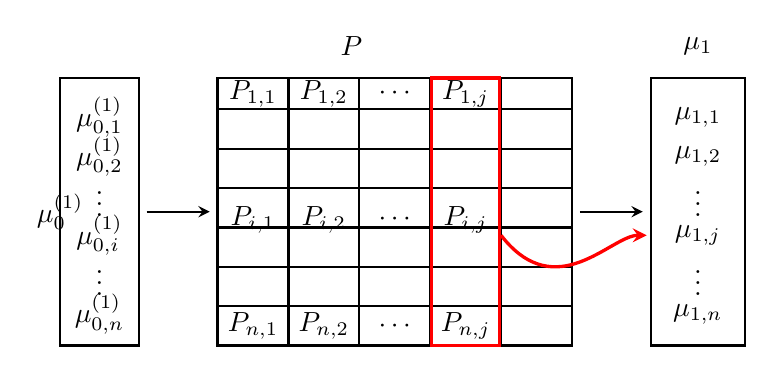
\begin{tikzpicture}[>=stealth, thick]

% Vettore mu_0
\node at (0,2.2) {$\mu_0^{(1)}$};
\draw (0,0.5) rectangle (1,3.9);
\foreach \y/\label in {3.4/$\mu_{0,1}^{(1)}$,2.9/$\mu_{0,2}^{(1)}$,2.4/$\vdots$,1.9/$\mu_{0,i}^{(1)}$,1.4/$\vdots$,0.9/$\mu_{0,n}^{(1)}$}
\node at (0.5,\y) {\label};

% Matrice P
\node at (3.7,4.3) {$P$};
\draw (2,0.5) rectangle (6.5,3.9);

% righe
\foreach \y in {1,1.5,2,2.5,3,3.5}
\draw (2,\y) -- (6.5,\y);

% colonne
\foreach \x in {2.9,3.8,4.7,5.6}
\draw (\x,0.5) -- (\x,3.9);

% elementi
\node at (2.45,3.7) {$P_{1,1}$};
\node at (3.35,3.7) {$P_{1,2}$};
\node at (4.25,3.7) {$\cdots$};
\node at (5.15,3.7) {$P_{1,j}$};

\node at (2.45,2.1) {$P_{i,1}$};
\node at (3.35,2.1) {$P_{i,2}$};
\node at (4.25,2.1) {$\cdots$};
\node at (5.15,2.1) {$P_{i,j}$};

\node at (2.45,0.75) {$P_{n,1}$};
\node at (3.35,0.75) {$P_{n,2}$};
\node at (4.25,0.75) {$\cdots$};
\node at (5.15,0.75) {$P_{n,j}$};

% freccia prodotto
\draw[->] (1.1,2.2) -- (1.9,2.2);
\draw[->] (6.6,2.2) -- (7.4,2.2);

% vettore mu_1
\node at (8.1,4.3) {$\mu_1$};
\draw (7.5,0.5) rectangle (8.7,3.9);

\node at (8.1,3.4) {$\mu_{1,1}$};
\node at (8.1,2.9) {$\mu_{1,2}$};
\node at (8.1,2.4) {$\vdots$};
\node at (8.1,1.9) {$\boxed{\mu_{1,j}}$};
\node at (8.1,1.4) {$\vdots$};
\node at (8.1,0.9) {$\mu_{1,n}$};

% evidenziazione colonna j
\draw[red, very thick] (4.72,0.5) rectangle (5.58,3.9);

% freccia dalla colonna j alla componente j
\draw[->, red, very thick] (5.6,1.9) .. controls (6.3,1.0) and (7.0,1.9) .. (7.45,1.9);

\end{tikzpicture}
\end{center}

La componente $j$-esima del prodotto $\mu_1=\mu_0^{(1)}P$ si ottiene prendendo la
\textbf{colonna $j$ di $P$} e facendo il prodotto scalare con $\mu_0^{(1)}$:

$$
\boxed{
\mu_{1,j}
=
\sum_{i=1}^{n}\mu_{0,i}^{(1)}P_{i,j}
}
$$

Quindi il significato degli indici è:

$$
\underbrace{P_{i,j}}_{\substack{\text{riga }i\\\text{colonna }j}}
$$

dove:

\begin{itemize}
\item $i$ indica quale componente di $\mu_0^{(1)}$ stiamo utilizzando;
\item $j$ indica \textbf{quale componente di $\mu_1$ vogliamo calcolare}.
\end{itemize}

In particolare, fissato $j$, percorriamo tutta la \textbf{colonna $j$ di $P$}:

$$
\boxed{
\mu_{1,j}
=
\mu_{0,1}^{(1)}P_{1,j}
+
\mu_{0,2}^{(1)}P_{2,j}
+\cdots+
\mu_{0,n}^{(1)}P_{n,j}
}
$$

\textbf{Stesso ragionamento viene fatto per $\mu_2$}, poi si mette in evidenza P ed esce:

\begin{align*}
(\mu_1 - \mu_2)_j &= \sum_{i=1}^n \left( \mu_{0,i}^{(1)} - \mu_{0,i}^{(2)} \right) P^\theta_{i,j} \\
&= \sum_{i=1}^n \left( \mu_{0,i}^{(1)} - \mu_{0,i}^{(2)} \right) \left[ (1 - n\alpha) Q_{i,j} + \alpha \right] \\
&= (1 - n\alpha) \sum_{i=1}^n \left( \mu_{0,i}^{(1)} - \mu_{0,i}^{(2)} \right) Q_{i,j} + \alpha \underbrace{\sum_{i=1}^n \left( \mu_{0,i}^{(1)} - \mu_{0,i}^{(2)} \right)}_{= 1 - 1 = 0} \\
&= (1 - n\alpha) \left[ \left( \mu_0^{(1)} - \mu_0^{(2)} \right) Q \right]_j
\end{align*}

Cioè:
\begin{equation}
    (\mu_1 - \mu_2) = (1 - n\alpha) \left[ \left( \mu_0^{(1)} - \mu_0^{(2)} \right) Q \right]
\end{equation}

\textit{Nota:} Il termine costante $\alpha$ si elide completamente poiché la somma dei pesi di una qualsiasi distribuzione di probabilità è sempre uguale a $1$.

\subsubsection*{3. Contrazione nella Distanza di Variazione Totale}
La metrica adottata per misurare la distanza tra distribuzioni è la \textit{Distanza di Variazione Totale} ($d_{TV}$) :
\begin{equation}
d_{TV}(\mu_1, \mu_2) = \frac{1}{2} \sum_{j=1}^n |\mu_{1,j} - \mu_{2,j}| = \frac{1}{2} \|\mu_1 - \mu_2\|_1
\end{equation}

Sfruttando la proprietà di non-espansione delle matrici stocastiche sotto norma $L^1$ (ovvero $\|v Q\|_1 \le \|v\|_1$), otteniamo:
\begin{align*}
d_{TV}(\mu_0^{(1)} P^\theta, \mu_0^{(2)} P^\theta) &= \frac{1}{2} (1 - n\alpha) \left\| \left( \mu_0^{(1)} - \mu_0^{(2)} \right) Q \right\|_1 \\
&\le (1 - n\alpha) \cdot \frac{1}{2} \left\| \mu_0^{(1)} - \mu_0^{(2)} \right\|_1 \\
&= (1 - n\alpha) \cdot d_{TV}(\mu_0^{(1)}, \mu_0^{(2)})
\end{align*}

e quindi :
\begin{equation}
    d_{TV}(\mu_0^{(1)} P^\theta, \mu_0^{(2)} P^\theta) <= (1 - n\alpha) \cdot d_{TV}(\mu_0^{(1)}, \mu_0^{(2)})
\end{equation}

\subsubsection*{4. Dimostrazione della Convergenza al Limite}
Definiamo il coefficiente $\gamma = (1 - n\alpha)$ . Poiché $\alpha > 0$ e $n \ge 1$, si ha che $0 \le \gamma < 1$, il che rende $\gamma$ un **fattore di contrazione** .

Iterando la catena per $k$ intervalli di ampiezza $\theta$ (corrispondenti al tempo $t = k\theta$):
\begin{equation}
d_{TV}(\mu_0^{(1)} P^{k\theta}, \mu_0^{(2)} P^{k\theta}) \le \gamma^k \cdot d_{TV}(\mu_0^{(1)}, \mu_0^{(2)}) \text{ dove } \gamma = 1-\alpha
\end{equation}

Poiché $\gamma < 1$, per $k \to \infty$ (e quindi per $t \to \infty$), il fattore $\gamma^k \to 0$ . Ne consegue che:
\begin{equation}
\lim_{t \to \infty} d_{TV}(\mu_0^{(1)} P^t, \mu_0^{(2)} P^t) = 0
\end{equation}
La distanza di variazione totale tende asintoticamente a zero, dimostrando che la catena di Markov converge verso una distribuzione stazionaria unica , indipendentemente dallo stato o dalla distribuzione iniziale .
\subsection{Applicazione al PageRank come Catena di Markov}

\paragraph{Formulazione del Modello di Navigazione}
Il PageRank modella la struttura del Web attraverso un grafo orientato $G = (V, E)$ in cui $|V| = N$ rappresenta l'insieme totale delle pagine web e $E$ la rete degli hyperlink.

Per superare i problemi matematici legati ai nodi pozzo (senza link uscenti) o a componenti disconnesse (spider traps), l'algoritmo introduce un \emph{damping factor} $\alpha \in (0, 1)$ (tipicamente impostato a valori quali $0.85$ o $0.75$).
\begin{itemize}
    \item Con probabilità $\alpha$, l'utente segue uno dei collegamenti ipertestuali uscenti dalla pagina corrente $s_i$, scelti con distribuzione uniforme $\frac{1}{r_i}$, dove $r_i$ indica il grado uscente (out-degree) della pagina $s_i$.
    \item Con probabilità $(1 - \alpha)$, l'utente interrompe la navigazione sequenziale ed effettua un salto casuale (\emph{teleportation}) verso una qualsiasi pagina del Web $N$ scelta uniformemente con probabilità $\frac{1}{N}$.
\end{itemize}

\paragraph{Matrice di Transizione Modificata}
La matrice di transizione globale del PageRank $P \in \mathbb{R}^{N \times N}$ ha componenti definite come:
\begin{equation*}
P_{i,j} = \begin{cases}
\alpha \cdot \frac{1}{r_i} + (1 - \alpha) \cdot \frac{1}{N} & \text{se esiste un link da } s_i \text{ a } s_j \\[8pt]
(1 - \alpha) \cdot \frac{1}{N} & \text{altrimenti}
\end{cases}
\end{equation*}

\paragraph{Dimostrazione di Ergodicità e Garanzia di Convergenza del PageRank}
L'aggiunta del termine di teletrasporto modifica la struttura della catena di Markov garantendo le seguenti proprietà formali:
\begin{enumerate}
    \item \textbf{Stretta Positività:} Poiché $\alpha < 1$ e $N \ge 1$, la quantità $(1 - \alpha)\frac{1}{N}$ è strettamente positiva per ogni coordinata. Ne consegue che:
    \begin{equation*}
    P_{i,j} > 0, \quad \forall i, j \in \{1, \dots, N\}
    \end{equation*}
    \item \textbf{Primitività con $\theta = 1$:} Essendo tutte le entrate della matrice $P$ strettamente positive già al primo passo ($\theta = 1$), la matrice $P$ è per definizione primitiva.
    \item \textbf{Irriducibilità ed Aperiodicità Implicite:} Il grafo associato a $P$ è una clique completa con archi orientati bidirectionali e cappi su ogni singolo nodo:
    \begin{itemize}
        \item Ogni nodo $s_i$ può raggiungere qualsiasi altro nodo $s_j$ in esattamente 1 passo ($\implies$ Irriducibilità).
        \item La presenza di self-loop ($P_{i,i} > 0$) implica $1 \in A_i \implies d(s_i) = \gcd(\{1, 2, \dots\}) = 1$ ($\implies$ Aperiodicità).
    \end{itemize}
    \item \textbf{Conclusione Matematica:} Il Teorema Fondamentale delle Catene Ergodiche assicura che il vettore del PageRank $\mu$ (la distribuzione stazionaria) \emph{esiste, è unico} ed è indipendente dalla configurazione iniziale $\mu_0$. Esso può essere calcolato numericamente tramite il metodo delle potenze (\emph{Power Method}):
    \begin{equation*}
    \lim_{t \to \infty} \mu_0 P^t = \mu
    \end{equation*}
    garantendo la convergenza algoritmica globale dell'architettura di ricerca.
\end{enumerate}


